\documentclass[a4paper ,12pt]{article}
\usepackage[colorlinks=true,linkcolor=black,urlcolor=blue,bookmarksopen=true]{hyperref}
\usepackage{bookmark}
\usepackage{fancyhdr} %Libreria para encabezado y pie de página.
\usepackage[utf8]{inputenc}
\usepackage{graphicx}
\graphicspath{ {graficos/} }

\usepackage{float}

\pagestyle{fancy} % Encabezado y pie de página
\fancyhf{}
\fancyhead[L]{TP2 - Grupo 25}
\fancyhead[R]{75.06 - Organización de Datos}
\renewcommand{\headrulewidth}{0.4pt}
\fancyfoot[C]{\thepage}
\renewcommand{\footrulewidth}{0.4pt}

\begin{document}
	
	
\tableofcontents % Índice general
\newpage

\section{Procesamiento y análisis de datos}\label{sec:intro}

En esta sección se introduce brevemente el producto a analizar y las herramientas que se utilizaron para realizar el análisis y la predicción requerida.



\subsection{Datos utilizados}

Se estudiaron datos provistos por la empresa Trocafone, analizando un conjunto de eventos de web analytics de usuarios que visitaron \url{www.trocafone.com}, su plataforma de e-commerce de Brasil.

\subsection{Sobre la empresa}

 
Trocafone es un side to side Marketplace para la compra y venta de dispositivos electrónicos que se encuentra actualmente operando en Brasil y Argentina. \\


La empresa realiza distintas actividades que van desde la implementación de plataformas de trade-in (conocidos en la Argentina como Plan Canje), logística directa y reversa, reparación y recertificación de dispositivos (refurbishing) y venta de productos recertificados por múltiples canales (ecommerce, marketplace y tiendas físicas).\\ 


Para conocer más de su modelo de negocio, pueden visitar el siguiente artículo:

\url{ https://medium.com/trocafone/el-maravilloso-mundo-de-trocafone-5bdc5761856b}

\subsection{Lenguajes y librerías utilizados}

\begin{itemize}
	
	\item Se utlizó como lenguaje de programación \textbf{Python3}.
	
	\item Para las visualizaciones, se utilizaron las librerías \textbf{ MatPlotLib }y\textbf{ Seaborn}.
	
	\item Como editor se utilizó \textbf{Jupyter Lab} (o \textbf{Jupyter Notebook})
	
	\item Para el manejo de DataFrames, se eligió \textbf{Pandas} como librería a utilizar.

	\item Se utilizaron algunas herramientas como std o argsort de la librería \textbf{Numpy}.
	calendar
	
	\item Se importaron diferentes métricas como "accuracy score", "f1 score", "precision score", "recall score", "roc auc score" de la librería \textbf{sklearn}.
	
	\item Se utilizaron diferentes busquedas de hiperparametros, entre ellas  "GridSearch" y "RandomizedSearchCV"  de \textbf{sklearn}.
	
	\item Para poder realizar cross-validation, se importó "StratifiedKFold" de \textbf{sklearn}.

	\item Se realizó Clustering mediante la funcion "KMeans" de la librería \textbf{sklearn}.
	
	\item Para la entrega final, los siguientes clasificadores fueron importados: 	"xgboost", "lightgbm", "RandomForestClassifier", "CatBoostClassifier".
	
	\item Se utilizo como ensamble de clasificadores a "VotingClassifier".
	
\end{itemize}

\subsection{Repositorio de Github}

Para el trabajo en conjunto del equipo, se utilizo un repositorio en github, donde se encuentran todos los archivos necesarios del análisis y predicciones y este informe propiamente dicho.\\

Link: \url{https://github.com/emabrea/7506-DATOS-TP2.git}

\newpage
\section{Breve análisis del set de Datos}
\subsection{Balance del set de datos}
Al haber muchas más visitas al sitio que compras de productos, el set de datos resulta ser muy desproporcionado, encontrándose muchas mas labels (95\%) con 0 (no compra) que 1 (compra). Esto es un gran problema para ciertos algoritmos de machine learning, que fallan con set de datos desbalanceados. 

Las soluciones a este problema son acotadas, ya que se dispone de un set de datos chico. Con la librería \textbf{imbalanced-learn} probamos distintas soluciones con oversampling, undersampling o combinaciones de ambos, pero no resultaron. 
Esto era lo esperado, ya que hacer oversampling significaría inventar la actividad de clientes, mientras que haciendo undersampling quedan muy pocos datos.

El problema se solucionó utilizando los parametros de los algoritmos de clasificación que permiten darle distinto peso a cada label. En particular, encontramos que la mejor relacion de pesos era de 1:7.

\subsection{Métrica usada}

Al tener el set de datos con 95\% de una clase, no se puede usar como métrica la precision, pues un algoritmo que solo arroje labels de esa clase, tendría un 95\% de precisión, a pesar de no predecir nada. Es por esto que se decidió utilizar otra métrica. En este caso, se utilizo el ROC AUC SCORE (Area Under Receiver Operating Characteristic Curve). En dicha métrica, se toman en cuenta los falsos positivos y negativos, y los verdaderos positivos y negativos. Con un random guess, se obtendría un 0.5, y con un puntaje perfecto, un 1.0. 
En la competencia, los valores altos se mantuvieron entre 0.85 y 0.88. Creemos que por la naturaleza del problema, sería muy difícil superar esa cota, pues puede haber dos usuarios con los mismos eventos, y uno compró y el otro no. 



\begin{figure}[H]
	\centering
	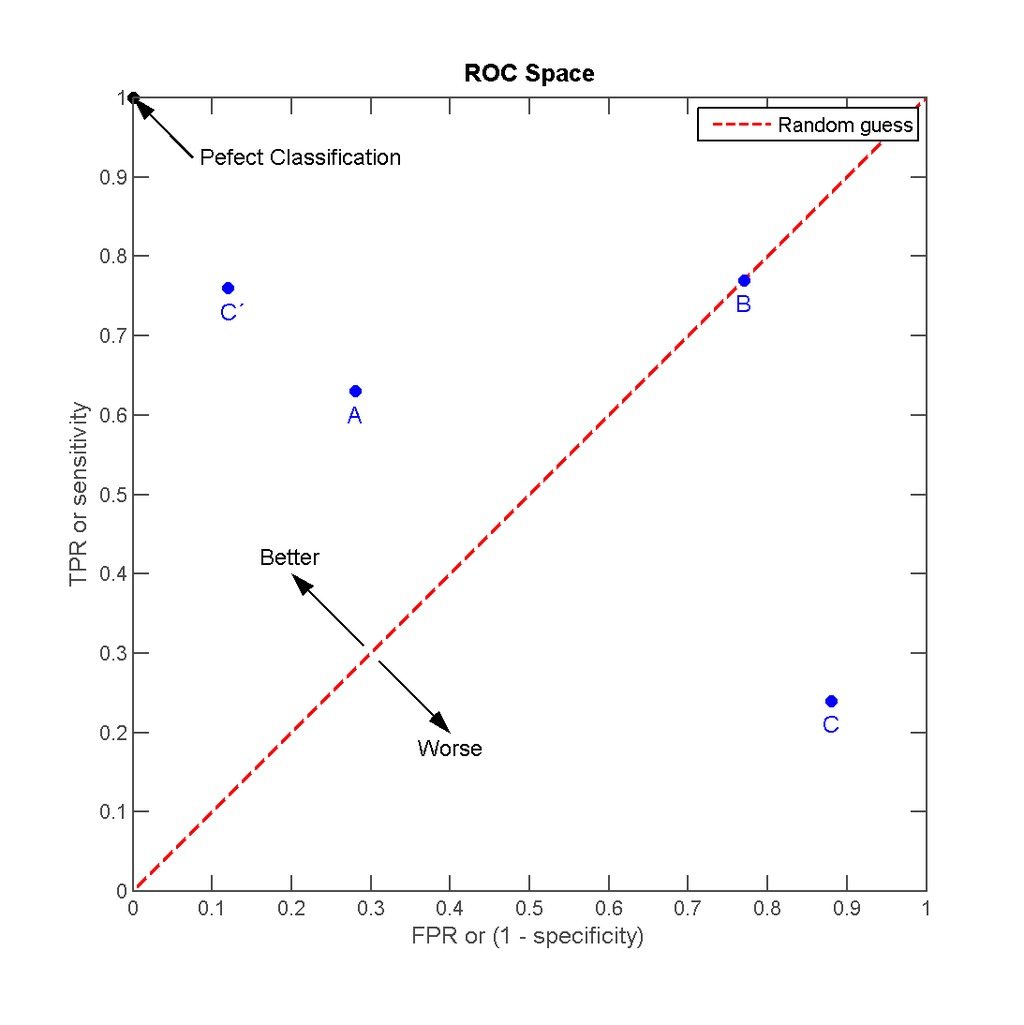
\includegraphics[width=1.1\textwidth, height=0.75\textheight]{roc_auc}
	\caption{\label{fig:01} Métrica usada }
\end{figure}

\begin{center}
	
\begin{figure}[H]
	\centering
	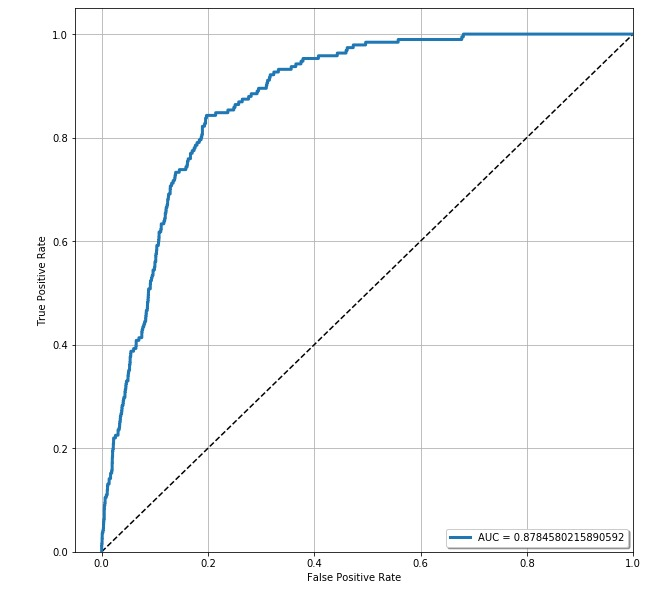
\includegraphics[width=1.1\textwidth , height=0.75\textheight]{roc_propia}
	\caption{\label{fig:02} Curva obtenida }
\end{figure}

\end{center}

\newpage
\subsection{Características interesantes a la hora de armar features}

Destacamos algunas características que pudimos extraer en un análisis previo mediante los siguientes gráficos:

\newpage

\begin{figure}[H]
\centering
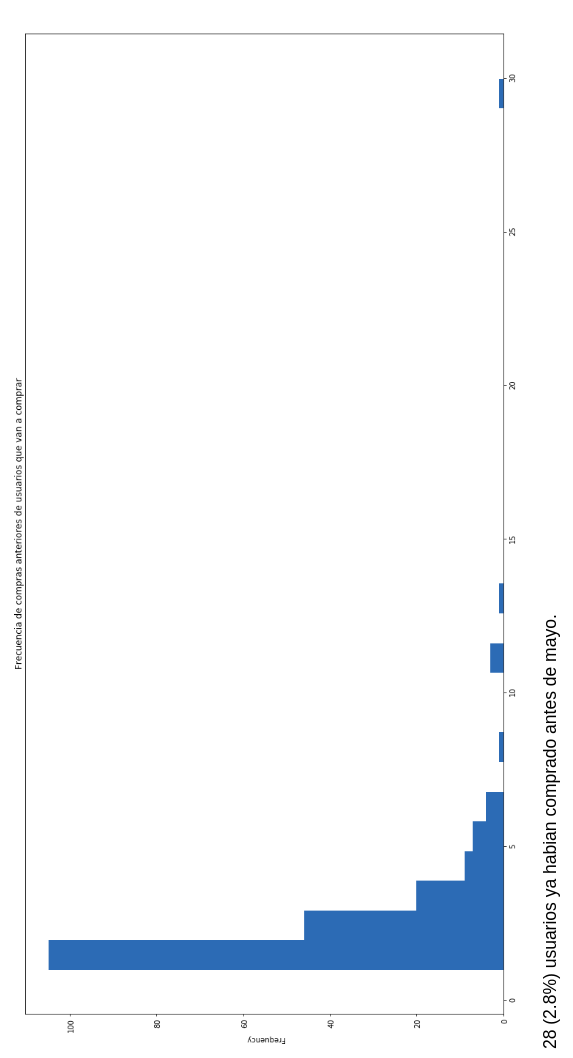
\includegraphics[width=\linewidth ,  height=0.95\textheight ]{compras_prev_a_compras}
\caption{Compras previas de los compradores de Junio}
\label{fig:compras_prev_a_compras}
\end{figure}

\begin{figure}[H]
\centering
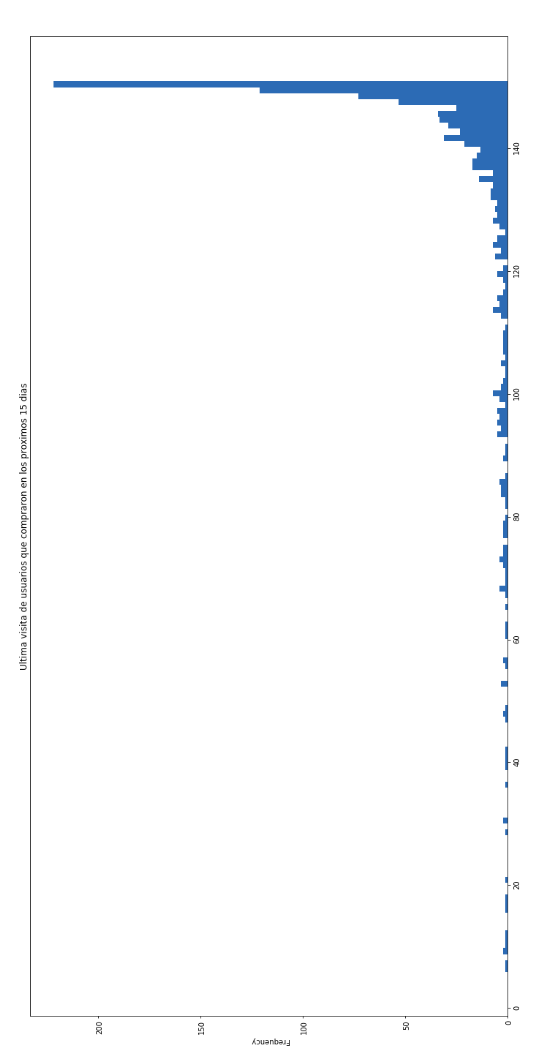
\includegraphics[width=\linewidth ,  height=0.95\textheight]{ult_vis_prev_com}
\caption{Ultima visita de compradores de Junio}
\label{fig:ult_vis_prev_com}
\end{figure}

\begin{figure}[H]
\centering
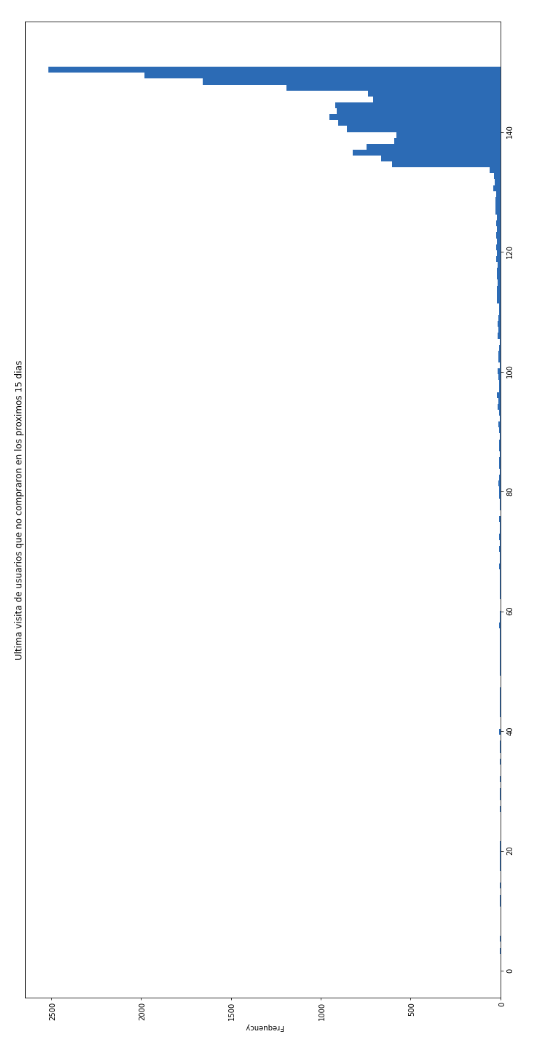
\includegraphics[width=\linewidth ,  height=0.95\textheight]{ult_vis_prev_no_compra}
\caption{Ultima visita de no-compradores de Junio}
\label{fig:ult_vis_prev_no_compra}
\end{figure}

\begin{figure}[H]
\centering
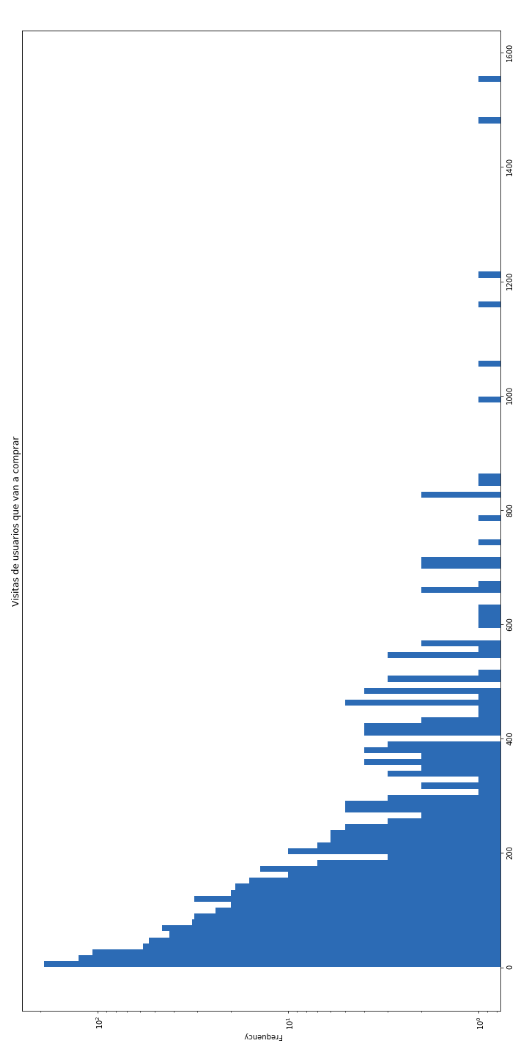
\includegraphics[width=\linewidth ,  height=0.95\textheight]{visitas_prev_compras}
\caption{Visitas previas de los compradores}
\label{fig:visitas_prev_compras}
\end{figure}

\begin{figure}[H]
\centering
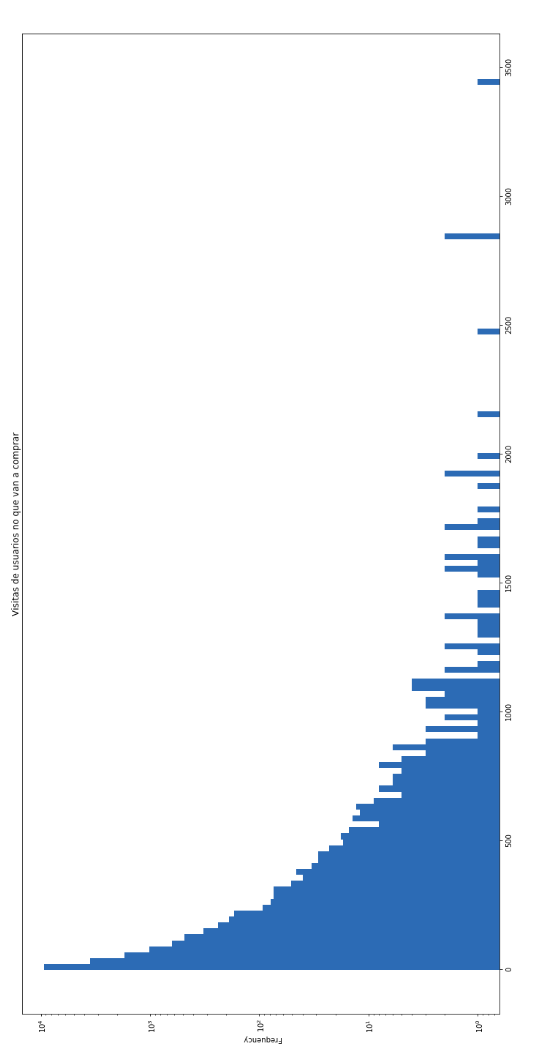
\includegraphics[width=\linewidth ,  height=0.95\textheight ]{visitas_prev_no_compras}
\caption{Visitas previas de los no compradores}
\label{fig:visitas_prev_no_compras}
\end{figure}


\newpage
\section{Featuring Engineering}

En esta sección hablaremos del aspecto más importante de nuestro algoritmo de Machine learning. Los features son determinantes a la hora de desarrollar un modelo predictivo. 

En nuestro modelo, como en la gran mayoría de los problemas de machine learning, la cantidad de features con la que contamos es simplemente mínima en comparación con los features que podemos crear a partir de los datos.
Para este problema en particular antes de pensar en la creación de fea-
tures tenemos que planificar cuál será nuestra estrategia para poder realizar las
predicciones que se nos piden y de qué forma vamos a entrenar nuestro modelo.

\subsection{Pensando en el modelo}

Para pensar en nuestro modelo debemos recordar que el objetivo es determinar para cada usuario presentado, cuál es la probabilidad de que ese usuario realice una conversión en Trocafone en un periodo determinado.

Es decir que nuestro modelo va a tener que procesar una serie de features que
dependen de columnas en un DataFrame de eventos hasta el 01/06/2018, este contenía principalmente variables categoricas y muchas columnas anuladas completamente.

Se listan a continuación: \\


\textbf{\underline{Columnas con valores no Nulos:}}

\begin{itemize}
	
	
	\item timestamp
	\item event 
	\item person 
	\item url 
	\item sku  
	\item model 
	\item condition 
	\item storage
	\item color 

	
\end{itemize}

\textbf{\underline{Columnas completamente de valores Nulos:}}

\begin{itemize}
	
		\item skus
		\item search term
		\item staticpage
		\item campaign source
		\item search engine
		\item hannel
		\item new vs returning
		\item city
		\item region
		\item country
		\item device type
		\item screen resolution
		\item operating system version
		\item browser version
		
\end{itemize}


Para validar el modelo podemos usar los datos provistos en un archivo .csv que contiene información de ciertos usuarios y si realizó una conversion en el periodo de tiempo el 01/06/2018 - 15/06/2018. \\

La construcción de features es un proceso creativo y la forma de validar si un
feature sirve o no es probando el modelo con nuestro set de validación, algunos
features pueden ser muy útiles, otros no tanto. \\

También se decidió agregar un archivo extra con recopilaciones propias de los precios de los moviles más visitados en el período del set de datos que se nos facilitó.


\subsection{Encoding}

El dataset contenía varias variables categóricas, las cuales no son aceptadas por
múltiples algoritmos de clasificación como por ejemplo XGBoost.

Otro problema es que a cada usuario se le debe asignar una sola muestra (fila), por lo tanto, surge el problema de que seleccionar luego de hacer el encoding. Por ejemplo, se puede codificar el almacenamiento de los modelos vistos, pero luego hay que asignarle uno solo a cada usuario. Es por esto que para este problema, encoding no fue muy útil.

Para poder utilizar las variables categóricas, se utilizaron los siguientes algoritmos:

\subsubsection{Count Encoding}
Consiste en reemplazar las categorías por la cantidad de
apariciones de las mismas en el set de datos. Resultó la codificación más simple de
implementar y fue la primera que utilizamos.

\subsubsection{One Hot Encoding}

Consiste en dividir el atributo en tantas columnas como valores posibles puede tener y usar cada columna como un dato binario indicando si el atributo toma o no dicho
valor. One-hot encoding es una codificación muy popular pero lamentablemente
no escala muy bien. En primer lugar es necesario construir en memoria un
diccionario por cada feature en donde asociaremos un número a cada posible
valor de cada columna, este diccionario puede ser demasiado grande. Otro
problema serio es que si una columna puede tomar muchos valores diferentes
posibles, por ejemplo la columna \textbf{model}, con $208$ representantes diferentes, entonces necesitamos cientos de nuevas columnas para representar los datos, esto hacía que ciertas a ciertas columnas ni siquiera se le intente aplicar dicho método ya que no es viable.


\subsubsection{Mean Encoding}
Esta codificación consiste en reemplazar las categorías con el
promedio de los valores a predecir en la categoría. Esto implica que por cada categoría, se calcula el promedio entre las postulaciones y no postulaciones y se
reemplaza la categoría por ese promedio. Esto se utilizo con los precios de los modelos, aplicandole el precio promedio a dichos eventos sin modelos (NaN).

\subsection{Featuring Engineering primera entrega (2º puesto)}

Llamamos entrega a un conjunto de mejoras que nos permitió no solo mejorar el score en Kaggle, sino incorporar varias mejoras en simultaneo.

Por la cantidad de submits realizados, decidimos en ocasiones agrupar varios submits con progresos bajo el nombre de una entrega.

\subsubsection{Primeros features}
Para el primer submit, se utilizaron unos 15 features, en su mayoria referidos al tiempo, como cantidad de visitas/ checkouts/ compras en los últimos X días. Con este sencillo enfoque, se obtuvo un puntaje de 0.85289 . Para las siguientes entregas, se uso el 100\% del set de datos, con más features, y mejores hiper-parametros. 

\subsection{Featuring Engineering segunda entrega (Train 100\%)}

\subsubsection{ Features sobre acciones por rango de tiempo }

		
		\subsubsection{Acciones en el último mes}
	
		\begin{itemize}
		 	
		\item Visitas último mes
		
		\item Checkouts último mes
		
		\item Compras último mes
		
		\item Subscripciones último mes
		\end{itemize}
		
	
		

		\subsubsection{Acciones en los últimos 15 días}		
		
		\begin{itemize}
			\item 	Visitas últimos 15
		\end{itemize}
		


		\subsubsection{Acciones en la última semana}
			
			\begin{itemize}
				\item  Visitas última semana
				\item  Checkouts última semana
				\item  Compras última semana 
				\item Campaña ultima semana
			\end{itemize}
			

		\subsubsection{Acciones en los últimos 3 días}
		
		
		
			\begin{itemize}
				\item Visitas últimos 3
			\end{itemize}





\subsubsection{Features de acciones del usuario}

	\begin{itemize}
		\item Total visitas usuario
		
		\item Total checkout
		
		\item Total compras
		
		\item Búsqueda celular 
		
		\item Días distintos 
		
		\item última visita 
		
	\end{itemize}
	


\subsubsection{Features de modelos}

	\begin{itemize}
		
		\item Modelos distintos vistos
			
	\end{itemize}	

\subsection{Featuring Engineering tercera entrega}

	Para esta entrega se decidió llevar a cabo el tuning del algoritmo (Sección 6).
	
	Para esto se realizó en primer lugar un Random-Search, con el fin de estimar los hiper-parametros óptimos o un intervalo al que pertenecía cada uno.
	
	Esto facilitó la posterior exhaustiva con Grid-Search, ya que pudimos reducir los intervalos de busqueda de la misma, y concentrarnos en obtener mejor precisión en los mismos.

\subsection{Featuring Engineering cuarta entrega}

	En esta ocasión surgió la necesidad del agregado de nuevos features, debido a que la elección de los algoritmos a ensamblar y sus hiperparametros tenía un impacto mucho menor que estos a la hora de mejorar el score.
	
\subsection{Cantidad de valores diferentes por característica}

\begin{itemize}
	\item horas distintas

	\item dias distintos ultima semana

	\item dias distintos de la semana

	\item dias distintos de la semana last month

	\item marcas distintas

	\item celular mas visto * (hablar de precios de celulares)

	\item compras por dia semana

	\item modelos por color

	\item eventos distintos

\end{itemize}

\newpage
\subsection{Featuring Engineering quinta entrega}

En la quinta entrega se decidió ir mas alla del set de datos provisto por el enunciado, debido a que se noto la ausencia de precios en 
los modelos de los equipos, es por eso que investigando en el sitio web de Trocafone, se decidió incluir los precios de los modelos más populares.

A continuación se muestra la lista de precios incluidos para entrenar el algoritmo:
Dicho esto, se decidió incluir los siguientes features representativos sobre el precio de los equipos en los eventos de cada usuario:

\begin{center}
	 	
		\begin{tabular}{lll}
			\hline
			Model&Capacidad(GB)&Precio \\
			\hline

			iPhone 5s&32&939 \\
			iPhone 5s&16&619 \\
			iPhone 6&16&949 \\
			iPhone 6&128&1499 \\
			iPhone 6&64&1069 \\
			iPhone 6 Plus&64&1769 \\
			iPhone 6 Plus&16&1589 \\
			iPhone 6S&64&1939\\
			iPhone 6S&32&1679\\
			iPhone 6S&16&1439\\
			iPhone 6S Plus&128&2199 \\
			iPhone 6S Plus&64&2089 \\
			iPhone 6S Plus&16&1959 \\
			iPhone 7&32&2229\\
			iPhone 7&128&2469\\
			iPhone 7&256&2819\\
			iPhone 7 Plus&128&3009 \\
			iPhone 7 Plus&256&3559 \\
			iPhone 7 Plus&32&2869 \\
			iPhone 8 Plus&64&4000 \\
			iPhone SE&64&1309 \\
			iPhone SE&16&999 \\
			iPhone X&64&5000 \\
			
		\hline
		\end{tabular}
	\\
	
	Tabla de celulares Iphone
\end{center}

\begin{center}
		
		\begin{tabular}{lll}
			\hline
			Model&Capacidad (GB)&Precio \\
			\hline
	
	LG G4 H818P&32&829 \\ 
	Motorola Moto X Style&32&950 \\
	Motorola Moto X2&16&569 \\
	Motorola Moto X2&32&619 \\
	Samsung Galaxy A7 2017&32&849 \\
	Samsung Galaxy A9 Pro 2016&32&1036 \\
	Samsung Galaxy J5&16&399 \\
	Samsung Galaxy J7 Prime&32&730 \\
	Samsung Galaxy S6 Edge Plus&64&2099 \\
	Samsung Galaxy S6 Flat&32&849 \\
	Samsung Galaxy S6 Flat&32&669 \\
	Samsung Galaxy S6 Flat&32&669 \\
	Samsung Galaxy S7&32&1089 \\
	Samsung Galaxy S7 Edge&32&1299 \\
	Samsung Galaxy S7 Edge&128&1479 \\
	Samsung Galaxy S8&64&1799 \\
	Samsung Galaxy S6 Edge&64&1039 \\
	Samsung Galaxy S6 Edge&32&900 \\
	iPhone 5c&8&450 \\
	Samsung Galaxy S8 Plus&64&1859  \\
	iPhone 5&16&550 \\
	Samsung Galaxy A5 2017&32&689 \\
	iPhone 4S&8&319 \\
	Samsung Galaxy J7&16&550 \\
	Motorola Moto X Play 4G Dual&4&599 \\
	Samsung Galaxy S5&16&439 \\
	Motorola Moto G3 4G&16&379 \\

		\hline
	\end{tabular}
	\\
	
	Lista de Moviles con su almacenamiento y precio correspondiente.

\end{center}


De la lista de precios de moviles se pudo extraer algunas características para ser tomadas como features:

\begin{itemize}
	\item Precio máximo
	\item Precio mínimo
	\item Desviación estandar de los precios
	\item Media de los precios
\end{itemize}

Con esta información, se pudo mejorar levemente el score, pero debido a la gran cantidad de NaN en la columna "Model", la mejora no fue la esperada.

\subsection{Featuring Engineering sexta entrega}

Se pudo observar en Select K-Best y en los feature importance de cada algoritmo que los features relacionados a Visitas, Checkouts y Conversion tenían un papel relevante a la hora de realizar predicciones, es por eso que se decidió intensificar la cantidad de features en dichas areas. Esto dió como resultado la inclusión de los siguientes:

\begin{itemize}
	
	\item visitas último día
	
	\item checkouts últimos 15 días
	
	\item checkouts últimos 3 días
	
	\item checkouts último día
	
	\item compras ultimos 3 días
	
	\item compras ultimos 15 días
	
	\item compras ultimo día
	
\end{itemize}

Sin embargo, para los submits finales, se usaron todos los features, pues observamos que aunque un feature no parezca importante para un algoritmo, eso no implica que quitandolo se mejore el resultado. 



\subsection{Featuring Engineering septima entrega}

		Siguiendo la corriente de pensamiento que nos llevó a la sexta entrega, se decidió reforzar los features con el agregado de los siguientes:	
		
	
\begin{itemize}
	

	\item visitas últimos 2 días 
	\item checkouts últimos 2 días
	\item checkouts últimos 4 días
	\item compras últimos 2 días
	\item compras últimos 5 días
	\item compras últimos 4 días
	
	
\end{itemize}

Es decir, se profundizo en características temporales, y haciendo varias segregaciones, se logró mejorar considerablemente el modelo, superando los 0.86. También se observo que el tipo de evento más "importante" para los algoritmos resulto ser el "checkout".
 
\section{Algoritmos de Clustering}

Luego de la clase sobre clustering, propusimos agregar como features los resultados de aplicar distintos algoritmos de clustering al set de datos. Se probó con K-means, K-means++, DBScan y HDBScan. Por prueba y error se fueron determinando los hiper parámetros k más convenientes. Tanto K-means como DBScan fueron posteriormente descartados ya que se notó que empeoraban los resultados.

Una posible interpretación de estos features es que estos algoritmos de clustering lograron identificar distintos grupos o sectores entre los visitantes al sitio, que ayudan a determinar si es probable o no que compren.

Features agregados:
\begin{itemize}
	\item k-means++, k=2
	\item k-means++, k=3
	\item k-means++, k=4
	\item k-means++, k=5
	\item k-means++, k=50
	\item k-means++, k=100
	\item HDBScan, k=100
\end{itemize}


\newpage
\section{Clasificadores utilizados}

En la ultima entrega se utilizó un Voting Classifier de cuatro algoritmos:

\begin{itemize}
	
	\item XGBoost
	
	\item Random Forest 
	
	\item LightGBM
	
	\item CatBoost
	
\end{itemize}

Sin embargo, esta elección provino de un arduo proceso de elecciones previas y combinaciones de algoritmos a ensamblar, a continuación listamos algunos de los algoritmos utilizados y la motivación para ir reemplazando las diferentes combinaciones por otras.

\begin{itemize}
	
	\item KNN
	
	Fue el primer algoritmo utilizado por su sencillez, pero no se pudo obtener más de 0.79 de score (local). Un problema es no poder indicarle el peso de las clases.
	
	\item Decision tree
	
	Primer algoritmo basado en arboles utilizado, pero debido a la naturaleza del problema (predicción de compras), no obtuvo buenos resultados. 
	
	\item Logistic regression
	
	A pesar de que es posible indicarle el peso de las clases, este algoritmo fallaba en encontrar los labels positivos. Se probaron varios valores de C, y del solver (newton-cg’, ‘lbfgs’, ‘liblinear’, ‘sag’, ‘saga’), pero no se pudo superar los 0.80.	
	
	\item SVM
	
	SVM acertaba muchos labels 0, pero muy pocos 1, por lo cual tenía muy buena precisión, pero un ROC AUC Score muy bajo. Se probaron varios kernel con distintos C, pero no resultó.
	
	\item Neural network 
	
	A este algoritmo se le dedicó mucho tiempo, con la esperanza de superar el puntaje obtenido. Para ello se normalizo (con varios métodos) todo el dataframe, y se trabajó con datos numéricos. 
	Se probaron diversos solvers (‘lbfgs’, ‘sgd’, ‘adam’), obteniendo mejores resultados con lbfgs. 
	Para la funcion de activación, se probaron: ‘identity’, ‘logistic’, ‘tanh’, ‘relu’, resultando mejor la funcion "relu".
	Luego, se probaron diversos valores de alpha, y de learning rate, como también varias capas (layers), entre 2 y 4. Esto aumento el tiempo del algoritmo, cuyo mejor resultado fue 0.8468. 
	Al hacer un ensamblador con otro algoritmo del tipo XGBoost, se obtuvieron buenos resultados, pero finalmente se decidió no incluirlo en la entrega final, entre otros motivos, por el tiempo tomado para entrenar.
	
	\item AdaBoost
	
	Este algoritmo dio buenos resultados, pero resulto ser un poco inferior a XGBoost, por lo cual, decidimos no incluirlo en el resultado final
	
	Como dato adicional, también se probo el famoso algoritmos Naive Bayes, pero como era de esperarse, los resultados no fueron buenos. 
	
	
	
\end{itemize}



\newpage
\section{Tuning}

En los diferentes algoritmos vamos a llamar parámetros a aquellos valores que el algoritmo encuentra a partir de los datos y vamos a llamar hiper-parámetros a
aquellos datos que el algoritmo necesita para poder funcionar.

Llamaremos óptimos a los hiper-parámetros que logren para un set de Datos maximizar determinada métrica, en este caso, utilizamos la métrica ROC AUC.\

Para encontrar los hiper-parámetros óptimos para un algoritmo pueden usarse dos métodos: Grid-Search o Random-Search.\\

\subsection{Grid-Search}

En un Grid-Search probamos todas las combinaciones posibles dentro de una lista de valores posibles para cada hiper-parámetro.

En este caso, debido a la cantidad de hiper-parámetros , se decidió comenzar en las listas de valores posibles para cada uno con un ”paso” grueso.

Esto reduce en un principio la cantidad de combinaciones a ejecutar. Luego se podra refinar la busqueda en la zona donde resultaron optimos nuestros hiper-parametros iniciales.

Este proceso fue especialmente necesario cuando los hiper-parámetros tomaban valores reales.

Cuando la cantidad de hiper-parámetros es realmente muy grande la combinatoria a realizar puede resultar muy ineficiente, en estos casos puede re-
currirse al método de Random-Search.

\subsection{Random-Search}

Como la cantidad de hiperparametros era elevada, posteriormente se recurrió al método de Random-Search,

En este método controlamos cuantas iteraciones realizamos de nuestro algoritmo y por cada iteración seleccionamos los valores de los
hiper-parámetros al azar dentro de un rango preestablecido. 

Cabe aclarar que este método no es tan preciso como un grid-search pero es mucho mas rápido, pudiendo invertir mayor parte del tiempo a la creación de Features.

\subsection{Aplicación a nuestro algoritmo}

En uno de nuestros primeros ensambles (constituídos por un Random Forest y un XGBoost) se aplico el método de Random Search con el fin de poder encontrar (u obtener una buena aproximacióń a ellos) de los hiperparametros:\\

\underline{Para XGBoost: }

\begin{itemize}
	\item scale pos weight (tipicamente: entre 3 y 9).
	\item learning rate (tipicamente: 0.001, 0.01, 0.05, 0.1)
	\item max depth (entre 1 y 6)
	\item n estimators (tipicamente: 500, 1000, 1500, 3000, 5000)
\end{itemize}



\underline{Para Random Forest:}

\begin{itemize}
	
	\item Peso de una de las clase 1 : La lista de este hiperparametro contenía los números del 3 al 10
	
	\item Criterio: Este hiper-parámetro podía ser : \{'gini', 'entropy'\}
	
	Y en general, para los demás algoritmos, también se probaron los mismos hiper-parametros que xgboost, como cantidad de árboles, profundidad, gamma, etc. 

\end{itemize}


Es muy importante aclarar que para la validación de hiper-parámetros se utilizó K-fold cross validation, con K= 10.

Es decir, de nuestro set de datos, el 10\% fue usado para validar los hiperparametros cada vez.


\newpage
\section{Ensamble}

Los mejores resultados en ML suelen surgir de la combinación de varios algo-
ritmos. Es muy raro que un solo algoritmo de ML logre mejores resultados que
un ensamble. Esto pudo verse en las sucesivas entregas, donde utilizar un ensamble nos traía resultados mas satisfactorios que usar los algoritmos individualmente.

\subsection{Combinando Algoritmos Diferentes}

Estos procesos suelen ser la clave para obtener un mejor resultado, ya que permitieron aprovechar el poder expresivo
de varios modelos completamente diferentes para obtener un resultado común.
En nuestro caso, el problema a abordar era de clasificación.

\subsubsection{Majority Voting}

Tenemos varios clasificadores distintos para un cierto problema, cada uno de ellos produce un resultado y queremos obtener un 
 resultado final. Una aproximación simple es ver cual es la clase que tiene mayoría entre todos los clasificadores.

En un primer momento, se decidió utilizar este tipo de ensamble debido a su simplicidad, 
pero nos encontramos que el mismo tiene sentido cuando la predicción es directamente la clase.
Si la predicción es la probabilidad de cada clase entonces obtuvimos que otros métodos funcionan mejor. 

Cuando la correlación entre los modelos es baja el resultado del ensamble, en general, mejora notablemente el resultado de cada modelo individual. 
\\

Una primera conclusión es que dados muchos clasificadores es conveniente elegir un conjunto que tenga buenos resultados y que estén muy poco correlacionados.

\subsubsection{Averaging}

Promediar el resultado de varios clasificadores es un método muy popular que
funciona en muchos problemas distintos: regresión, clasificación (ya sea para
predecir clases o probabilidades), etc. La idea principal es reducir el overfitting.

En general, una separación suave entre las clases es mejor que una separación
muy irregular y promediar clasificadores logra esto.

Cuando promediamos clasificadores que predicen la probabilidad de las clases, hubo
que prestar especial atención porque cada clasificador individual puede tener una calibración completamente diferente. 

Uno puede dar probabilidades muy cercanas a 1s y 0s mientras que otro, a lo mejor, se mantiene dentro de un cierto rango.
Una solución para esto es convertir cada probabilidad de un rango entre 1 y n, siendo n el total de personas a predecir. La persona con mayor probabilidad tiene 1,
el segundo 2, etc, y el de menor probabilidad, n, sin importar el valor de las probabilidades. Si hacemos esto para todos los clasificadores podemos luego
promediar los rangos y convertir estos promedios en un número entre 0 y 1 para la probabilidad final.

\newpage
\subsection{Aplicación a nuestro algoritmo}

Luego de 15 días de pruebas cuasi-continuas con algoritmos "individuales", se decidió emprender el camino de un ensamble, que pudiera extraer la expresividad particular de los mejores (según score en Kaggle) algoritmos  algoritmo utilizado hasta el momento.

Esto nos llevó a multiples combinaciones y elecciones de los algoritmos a ensamblar y el ensamblador, en donde emergió la función \textbf{ VotingClassifier} de la librería \textbf{sklearn.ensemble} como principal candidato a ensamblador.


\subsubsection{VotingClassifier}

La idea detras de VotingClassifier es la de combinar conceptualmente diferentes clasificadores de Machine Learning y usar \textit{mayoría simple} o un \textit{promedio suave} (soft vote) de las probabilidades predecidas por cada metodo para realizar la predicción de probabilidad. Un clasificador de este estilo pretende balancear los diferentes algoritmos de tal manera de minimizar los puntos debiles de cada uno.


\subsubsection{Elección final}

En un primer momento se realizaron diversas corridas de prueba en las que el promedio suave predominaba notablemente ante la mayoría simple, por lo que se decidió de ahi en adelante, usar la versión \textit{soft} de nuestro algoritmo.

Para las elección de los algoritmos, notamos que necesitabamos algoritmos que se destaquen en aspectos diferentes, y luego de una exhaustiva busqueda se decidió utilizar los siguientes:

\begin{itemize}
	\item XGBoost
	
	\item Light GBM
	
	\item Random Forest
	
	\item CatBoost

\end{itemize}

Estos algoritmos en conjunto lograron mas riqueza en la expresividad, y permitieron alcanzar scores más gratificantes que los obtenidos individualmente.

\newpage

\section{Últimas entregas}
	
	Cabe aclarar que los features y comentarios se realizaron hasta la 10ma entrega, que arrojó nuestro máximo
	
	
	En las últimas entregas se buscó enriquecer el modelo en terminos de features, constatando caso por caso que nuestro ensamble era quien mejores resultados arrojaba.\\
	
	Cabe destacar que la mayoría de los features están relacionados a aspectos temporales.\\
	
	Con esto se llegó a aproximadamente un conjunto de 80 features, y se muestran a continuación el feature importance de algunos features para algunos algoritmos.
	
	Se listan a continuación algunos de los features agregados en las últimas entregas:
	
	\begin{itemize}
		\item checkouts ultimos 16
		\item checkouts ultimos 17
		\item checkouts ultimos 18
		\item checkouts ultimos 19
		
		$\cdots$
	
	\end{itemize}
	
	y así con diferentes días, sorprendiendonos que en el feature importance de XGBoost se destacaba \textit{ checkouts ultimos 16} como el de mayor importancia.
	
	
	\begin{figure}
\centering
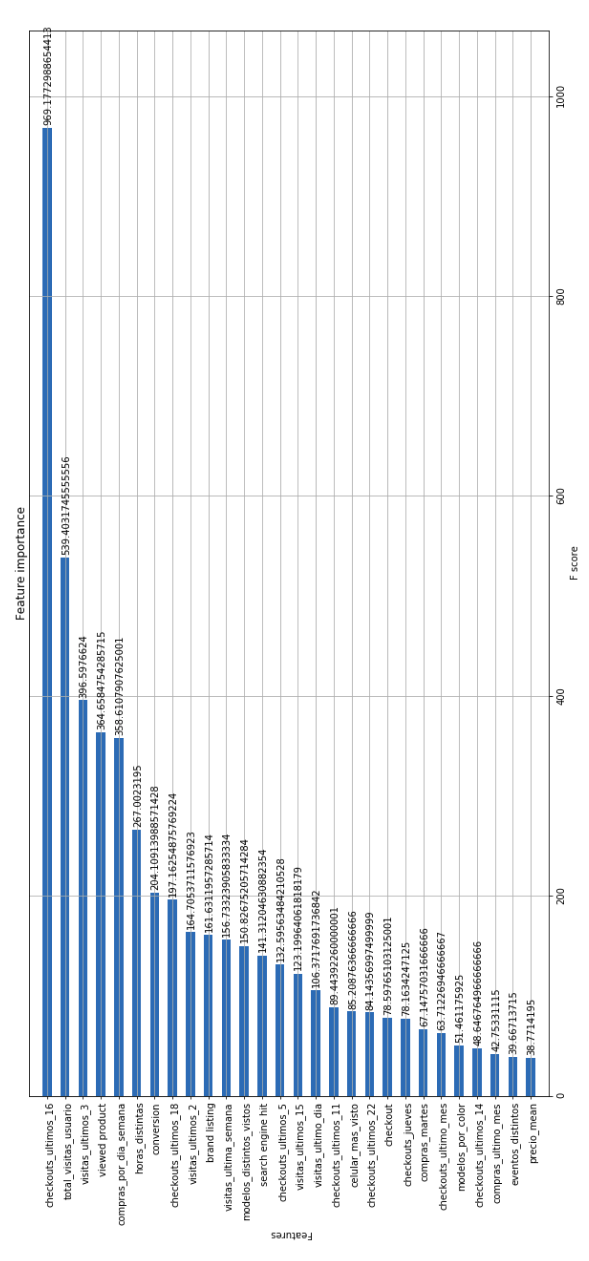
\includegraphics[width=\linewidth , height=0.9\textheight]{feature-XGB}
\caption{Feature importance XGBoost}
\label{fig:feature-XGB}
\end{figure}


Se muestra a continuación un gráfico del feature importance de Random Forest, que numera los features con la aparición en el DataFrame:

\begin{figure}
\centering
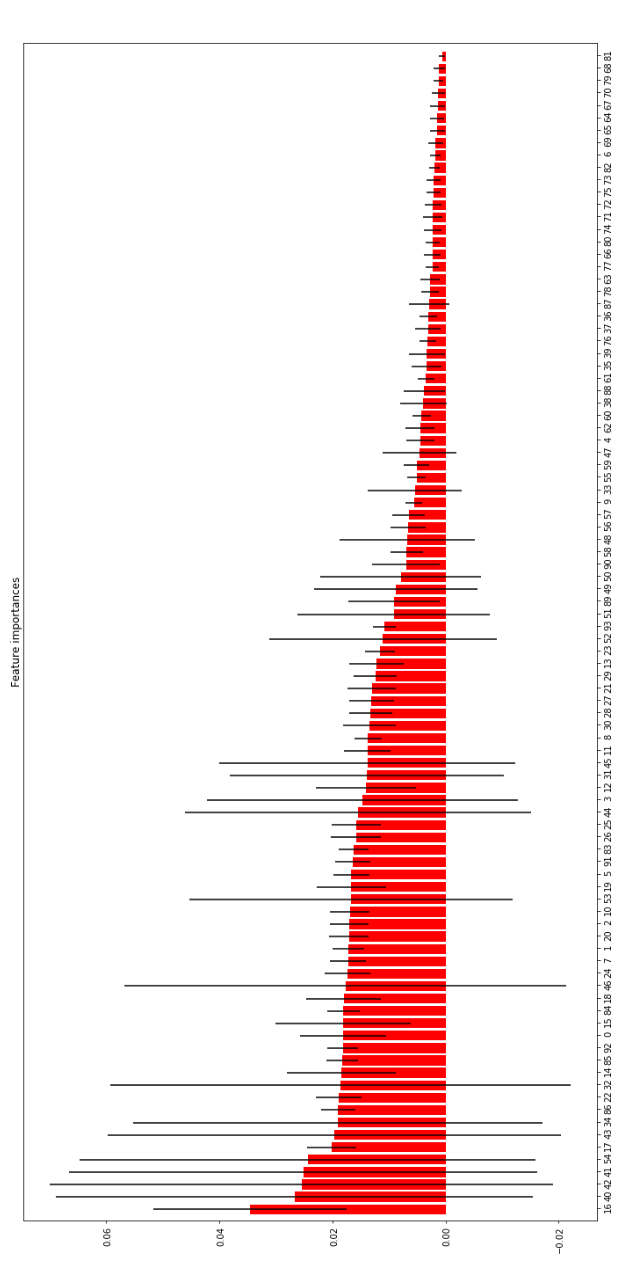
\includegraphics[width=0.8\linewidth,  height=0.9\textheight]{feature-RF}
\caption{Feature Importance de Random Forest}
\label{fig:feature-RF}
\end{figure}
	
Tambien se buscó relacionar el día de la semana con la cantidad de un evento de tal tipo, dando origen a features del estilo:

	\begin{itemize}
		\item 	checkouts viernes
		
		\item compras jueves
		
		$\cdots$
	\end{itemize}	

	
	
	Tambien decidimos mencionar que hubo intentos descartados de poder fabricar features con diversos eventos, como por ejemplo \textit{Brand Listing y Search Product}, que quedaron en codigo Markdown como evidencia que se intentó proceder con ellos en algún momento
	
\newpage

\section{Tiempos de ejecución}

	Los tiempos de ejecución de nuestros algoritmos no nos representaron un problema a lo largo de la inspección de nuevos features y clasificadores. Estos nunca fueron superiores a los veinte minutos.\\
	
	Como comentario, el algoritmo completo tarda poco menos de 20 minutos en completar su ejecución (incluyendo entrenamiento).
	
	
	\subsection{Tiempos de ejecución de Tuning}
	
	Cabe destacar que en el Tuning se registraron tiempos extremadamente altos (en particular en el Grid-Search) pero siempre controlados previamente por los alumnos mediante estimaciones.\\
	
	\subsubsection{Random Search}
	
	Se ejecutó reiteradas veces el algoritmo de Random-Search, controlando su cantidad de ejecuciones de manera de tardar a lo sumo 2 horas, esto nos permitió reducir el scope de busqueda mediante Grid Search, con el fin de obtener resultados más precisos.\\
	
	\subsubsection{Grid Search}
	
	Se ejecutó en dos ocasiones (relevantes) el algoritmo de Grid Search, con un promedio de ejecución de 14 horas cada uno, con el fín de obtener los hiperparametros con la máxima exactitud posible.

\newpage

\section{Conclusiones Generales}

Luego de todo el trabajo realizado, y teniendo en consideración aquellos intentos con algoritmos y features no incluidos en este informe, nos pareció importante destacar las siguientes conclusiones:


	\begin{itemize}
		
		\item La busqueda de features es una tarea creativa, pero a su vez ardua, ya que depende de cada problema en particular y como estén dispuestos los datos en el mismo.
		
		\item Si es posible tener alguna métrica para algún algoritmo, será importante reforzar o agregar features similares a los que el algoritmo considera como más usados.
		
		\item Pese a que agregar features en general ayuda, muchas veces es necesario tambien filtrar features que no son tan utilizados, con el fín de resaltar los demás.
		
		\item Ante columnas con variables categóricas, es crucial realizar encodings correspondientes, ya que las mismas aportan información útil en la mayoría de los casos ( en nuestro problema, la gran mayoría de columnas eran de este estilo).
		
		\item Combinar algorimos con expresividades variadas dentro de un ensamblador que permita maximizar las fortalezas de cada uno, y disminuir las debilidades.
		
		
		
	\end{itemize}
	
\newpage


\begin{thebibliography}{99}
		
	\bibitem{}Trocafone website, \url{www.trocafone.com}.
	
	\bibitem{} NumPy - NumPy, \url{http://www.numpy.org/}.
	
	\bibitem{} Python Data Analysis Library,
	\url{https://pandas.pydata.org/}.
	
	\bibitem{}	Matplotlib: Python plotting — Matplotlib 3.0.0 documentation,
	\url{matplotlib.org}.


	\bibitem{} XGBoost documentation,

	\url{
	https://xgboost.readthedocs.io/en/latest/parameter.html}

	\bibitem{} Random Forest documentation,

	\url{
	https://scikit-learn.org/stable/modules/generated/sklearn.ensemble.RandomForestClassifier.html}

	\bibitem{} Light GBM documentation,

	\url{
	https://github.com/Microsoft/LightGBM/blob/master/docs/Parameters.rst}

	\bibitem{} CatBoost documentation,
	
	\url{
	https://github.com/catboost/catboost}

	\bibitem{} Voting Classifier documentation,

	\url{
	http://scikit-learn.org/stable/modules/generated/sklearn.ensemble.VotingClassifier.html#sklearn.ensemble.VotingClassifier}
	
	\bibitem{} HDBScan documentation,
	
	\url{
		https://hdbscan.readthedocs.io/en/latest/how\_hdbscan\_works.html}

	\bibitem{} Select K best features documentation,
	
	\url{
		https://scikit-learn.org/stable/modules/generated/sklearn.feature\_selection.SelectKBest.html}
	
	\bibitem{} KNN documentation,
	
	\url{
		https://scikit-learn.org/stable/modules/generated/sklearn.neighbors.KNeighborsClassifier.html}
	
	\bibitem{} Decision tree documentation,
	
	\url{
			http://scikit-learn.org/stable/modules/generated/sklearn.tree.DecisionTreeClassifier.html}
		
	\bibitem{} Logistic regression documentation,
		
	\url{
			https://scikit-learn.org/stable/modules/generated/sklearn.linear\_model.LogisticRegression.html}
		
	\bibitem{} SVM documentation,
	
	\url{
		https://scikit-learn.org/stable/modules/generated/sklearn.svm.SVC.html}
	
	\bibitem{} Neural network documentation,
	
	\url{
		https://scikit-learn.org/stable/modules/generated/sklearn.neural\_network.MLPClassifier.html}
	
	
	
	







	

	
\end{thebibliography}


\end{document}
